\subsection{Markovian model without latent variables} \label{simple_generative_model}

% Design of the prior and optimization
\subsubsection{Design of the prior}

% Design

We aim at defining a parameterized distribution $p_{\theta}(T)$ from which one can sample trees.
We would also like this distribution to model the trees of the microbiota dataset, meaning that
the generated trees should look like the ones from the dataset as well, and respect the phylogenetic constraints. \\

\newcommand{\nodeparent}{\mathcal{P}}

Consequently, we introduce a first simple generative process to characterize $p_{\theta}(T)$ that we would call the markovian parenting tree generator.
Before describing the generation method, let us introduce the framework of it:
\begin{itemize}
    \item Describe $T$ as a succession of $L$ layers: $T = (T^{(1)}, \dots, T^{(L)})$.
    We assume that we have no missing data, so to say, all the leaves the tree are reaching the precision layer $L$.
    \item Describe a given layer $l$ as a discrete vector in $\{0, 1\}^{U}$.
    To each possible node at layer $l$ we can associate an index $k$ so that we denote the nodes by $u_k^{(l)} \in \{0, 1\}$.
    A node $u_k^{(l)}$ is activated if it is valued as $1$ in $T^{(l)}$, otherwise it is not.
    \item We introduce the function $\nodeparent$ that takes a node $u_k^{(l)}$ as input, and output the parent of the node if it is well defined in $T$,
          otherwise it outputs $0$ as if the parent was not activated:
            $$
            \nodeparent(u_k^{(l)}) = \left\{
            \begin{array}{ll}
                1 & \mbox{if } \text{parent of $u_k^{(l)}$ exists and is activated}\\
                0 & \mbox{otherwise}
            \end{array}
            \right.
            $$
\end{itemize}

Now that the framework is clear and defined, we describe the generative process:
\begin{itemize}
    \item The root node of the tree is deterministic, since all trees begin to the same root ancestor.
    Hence, we have:
    $$
    p(T^{(1)}) = \mathds{1}_{T^{(1)} = e_1}
    $$

    \item For all $l \geq 2, k \in \{1, \dots, U\}$, we assume that the activation of the node $u_k^{(l)}$
        is distributed as a Bernoulli conditionally to its parent activation, parameterized by $\pi_k^{(l)}$:
        $$
        u_k^{(l)} | \left \{\nodeparent(u_k^{(l)}) = 1 \right\} \sim \mathcal{B}(\pi_{k}^{(l)})
        $$
        To respect the tree architecture, we assume that if $\nodeparent(u_k^{(l)}) = 0$ then the probability for the children
        to be activated is deterministic and set to $0$, as a child can not exist without his parent.
    \item For now, we make the major assumption that all nodes are independent within a given layer conditionally to their parents, and they only depend on their respective parent, so that:
    $$
    \begin{align}
        p\left(u_1^{(l)}, \dots, u_K^{(l)} | \nodeparent(u_1^{(l)}), \dots, \nodeparent(u_K^{(l)}) \right) &= \prod_{k=1}^{K} p\left(u_k^{(l)} | \nodeparent(u_k^{(l)})\right)
    \end{align}
    $$

    \item The dependency between the layers of the tree is markovian:
    $$
    p_{\theta}(T^{(l+1)} | T^{(1:l)}) = p_{\theta}(T^{(l+1)} | T^{(l)})
    $$
\end{itemize}

Noting these framework properties, we can describe the distribution of such prior model on the trees:
$$
\begin{align}
    p_{\theta}(T) &= p_{\theta}\left(T^{(1)}, \dots, T^{(L)}\right) \\
    &= p\left(T^{(1)}\right) \prod_{l=1}^{L-1} p_{\theta}\left(T^{(l+1)}|T^{(l)}\right) \\
    &= \mathds{1}_{T^{(1)} = e_1} \prod_{l=1}^{L-1} p\left(u_1^{(l+1)}, \dots, u_K^{(l+1)} | \nodeparent(u_1^{(l+1)}), \dots, \nodeparent(u_K^{(l+1)})\right) \\
    &= \mathds{1}_{T^{(1)} = e_1} \prod_{l=1}^{L-1} \prod_{k=1}^K p\left(u_k^{(l+1)} | \nodeparent(u_k^{(l+1)}) \right) \\
    &= \mathds{1}_{T^{(1)} = e_1} \prod_{l=1}^{L-1} \prod_{k=1}^K \underbrace{\nodeparent(u_k^{(l+1)})}_{\text{$1$ if node has parent}} \left(\underbrace{u_k^{(l+1)}}_{\text{$1$ if activated}} \pi_k^{(l+1)} + (1-u_k^{(l+1)}) (1-\pi_k^{(l+1)}) \right)
\end{align}
$$

Looking at the previous formula, we obtain that such prior is parameterized by the activation probabilities $\pi_k^{(l)}$ of each node $u_k^{(l)}$.
Furthermore, due to the indicator function expressed through $\nodeparent(u_k^{(l+1)})$, the update of a given activation probability
will only be impacted by the trees which have the node $u_k^{(l)}$ in any branch. \\

% Optimization
Now that the prior of the trees is well defined, we would like to compute an optimal value of
$\pi^{(l)} = \left(\pi_1^{(l)}, \dots, \pi_{U}^{(l)}\right)$ in the sense of the maximum of likelihood. \\
The maximum log-likelihood objective for $\pi_k^{(l)}$ over our microbiota dataset can then be written as:
$$
\begin{equation}
    \begin{align}
        \left(\pi_j^{(m)}\right)^* = arg \max_{\pi_j^{(m)}} \quad & \sum_{i=1}^n \mathds{1}_{T_i^{(1)} = e_1} \sum_{l=1}^{L-1} \sum_{k=1}^K \nodeparent(u_{k,i}^{(l+1)}) \left[u_{k,i}^{(l+1)} \log \pi_{k}^{(l+1)} + (1 - u_{k,i}^{(l+1)}) \log (1 - \pi_k^{(l+1)}) \right] \\
        \textrm{s.t.} \quad & \forall k, \pi_{k}^{(L)} \in [0, 1] \\
    \end{align}
    \label{eq:prior_transition_objective}
\end{equation}
$$

Then, simply by deriving the log-likelihood we obtain:
$$
\begin{align}
    \partial_{\pi_j^{(m)}} \log p(T_1, \dots, T_n) &= \sum_{i=1}^n \mathds{1}_{T_i^{(1)} = e_1} \nodeparent(u_{j,i}^{(m)}) \left[ u_{j,i}^{(m)} \frac{1}{\pi_j^{(m)}} + (1 - u_{j,i}^{(m)}) \frac{-1}{1-\pi_j^{(m)}}\right] \\
                                                    &= \frac{1}{\pi_j^{(m)}} \sum_{i=1}^n \mathds{1}_{T_i^{(1)} = e_1} \nodeparent(u_{j,i}^{(m)}) u_{j,i}^{(m)} - \frac{1}{1 - \pi_j^{(m)}} \sum_{i=1}^n \mathds{1}_{T_i^{(1)} = e_1} \nodeparent(u_{j,i}^{(m)}) (1 - u_{j,i}^{(m)})
\end{align}
$$

Looking for $0$ valued gradient, we end up with:
$$
\begin{align}
    (1 - \pi_j^{(m)}) \sum_{i=1}^n \mathds{1}_{T_i^{(1)} = e_1} \nodeparent(u_{j,i}^{(m)}) u_{j,i}^{(m)} - \pi_j^{(m)} \sum_{i=1}^n \mathds{1}_{T_i^{(1)} = e_1} \nodeparent(u_{j,i}^{(m)}) (1 - u_{j,i}^{(m)}) &= 0 \\
    \pi_j^{(m)} \sum_{i=1}^n \mathds{1}_{T_i^{(1)} = e_1} \nodeparent(u_{j,i}^{(m)}) &= \sum_{i=1}^n \mathds{1}_{T_i^{(1)} = e_1} \nodeparent(u_{j,i}^{(m)}) u_{j,i}^{(m)} \\
    \pi_j^{(m)} &= \frac{\sum_{i=1}^n \mathds{1}_{T_i^{(1)} = e_1} \nodeparent(u_{j,i}^{(m)}) u_{j,i}^{(m)}}{\sum_{i=1}^n \mathds{1}_{T_i^{(1)} = e_1} \nodeparent(u_{j,i}^{(m)})}
\end{align}
$$

Since the previous quantity respects the constraint to be in $[0,1]$,
we obtain the optimal activation probability for every bacteria as:
$$
\fbox{
    \displaystyle
    \left(\pi_k^{(l)}\right)^* &= \frac{\sum_{i=1}^n \mathds{1}_{T_i^{(1)} = e_1} \nodeparent(u_{k,i}^{(l)}) u_{k,i}^{(l)}}{\sum_{i=1}^n \mathds{1}_{T_i^{(1)} = e_1} \nodeparent(u_{k,i}^{(l)})}
}
$$

This estimator is actually the common MLE for a Bernoulli parameter estimation, except that it limits
the computation of the estimation to all trees that respect the root constraint, and that could possess the node $u_k^{(l)}$
since they must have the parent node $\nodeparent(u_k^{(l)})$.

% Design of the posterior and optimization
\subsubsection{Design of the posterior and maximum likelihood estimator}

\newcommand{\childrennode}{\mathcal{C}}

% Design of the posterior

Now that we have a way to generate trees, we need to define an explicit stochastic relationship between the abundance
data and the structure of the tree.
Such inevitably exists, as when observing $T$, the abundance of an entity that isn't present in $T$ is necessarily 0.
Similarly, it is highly likely that when observing the presence of certain entities in $T$ that induces a high abundance of
another neighbour entity (interaction between bacteria). \\

For context, we recall that $X$ is a matrix of shape $(L, U)$,
where $L$ is the maximum precision level of the trees (assumed to be the same for all trees for now) and $U$ the maximum number of entities at each depth of the trees.
We denote by $X^{(l)}$ the $l$-th line of the abundance matrix, for which up to $U_l$ elements should be non-zero. \\

We assume the following framework:
\begin{itemize}
    \item We denote $X^{(l)} = (x_1^{(l)}, \dots, x_U^{(l)})$ the abundance vector at layer $l$.
    \item For an abundance node $x_k^{(l)}$, we denote by $\childrennode(x_k^{(l)})$ the set of abundance children associated to that node.
    \item $X^{(1)} = [1, 0, \dots, 0]$, since it's the root of the tree, only one entity gets the whole weight.
    \item Since we would like a simple explicit model at first, we design a posterior $p_{\theta}(X|T)$ which is markovian relatively to the layers of the tree,
            so that the abundance at the next layer are only impacted by the previous layers abundance for now:
            $$
            p_{\theta}(X^{(l)} | X^{(1:l-1)}, T) = p_{\theta}(X^{(l)} | X^{(l-1)}, T)
            $$
    \item Each value in $X^{(l)}$ is restricted by the following set of constraints:
            \begin{itemize}
                \item If node $k$ at layer $l-1$ has one child, then its abundance value is the same for the child node.
                \item If node $k$ at layer $l-1$ has at least two children, the children abundance sums to the parent's abundance value.
            \end{itemize}
    \item Since we deal with proportions in abundance vectors, it seems natural to use the Dirichlet distribution in first assumption.
          Hence, we assume that for all $l \geq 2$, if $|\childrennode(x_k^{(l)})| > 1$,
            $$\childrennode(x_k^{(l)}) | x_k^{(l)}, T \sim \mathcal{D}(\alpha_k^{(l)})$$
          We denote by $f_{\alpha_k^{(l)}}$ the density of this distribution, parameterized by $\alpha_k^{(l)}$.
          Notice that setting this distribution framework enables us to verify the constraints given above by renormalizing the layer with the obtained weights.
          Naturally, if $|\childrennode(x_k^{(l)})| = 1$, we have $\childrennode(x_k^{(l)}) \sim \delta_{x_k^{(l)}}$.
\end{itemize}

Noting the previous framework, the whole abundance distribution conditionally to the trees is then given by:
$$
\begin{align}
    p_{\theta}(X | T) &= \prod_{i=1}^n p_{\theta}(X_i | T_i) \\
    &= \prod_{i=1}^n p_{\theta}(X_i^{(1)}, \dots, X_i^{(L)} | T_i) \\
    &= \prod_{i=1}^n p(X_i^{(1)} | T_i) \prod_{l=1}^{L-1} p_{\alpha_l}(X_i^{(l+1)} | X_i^{(l)}, T_i) \\
    &= \prod_{i=1}^n \mathds{1}_{X_i^{(1)} = e_1} \prod_{l=1}^{L-1} \prod_{k=1}^U p(\childrennode(x_{k,i}^{(l)}) | x_{k,i}^{(l)}) \\
    &= \prod_{i=1}^n \mathds{1}_{X_i^{(1)} = e_1} \prod_{l=1}^{L-1} \prod_{k=1}^U \left[\mathds{1}_{|\childrennode(x_{i,k}^{(l)})| = 1} \mathds{1}\left(\childrennode(x_{k,i}^{(l)}) = x_{k,i}^{(l)}\right) + \mathds{1}_{|\childrennode(x_{i,k}^{(l)})| > 1} f_{\alpha_k^{(l)}}\left(\childrennode(x_{k,i}^{(l)})\right)\right]
\end{align}
$$

% Optimization

This distribution is parameterized at each layer $l$ by $\alpha^{(l)} = (\alpha_1^{(l)}, \dots, \alpha_U^{(l)})$, the various Dirichlet parameters of the layers of the tree.
Hence, the optimization objective can be written as:
$$
\begin{equation*}
    \begin{align}
        \left(\alpha_{j,v}^{(m)}\right)^* = arg \max_{\alpha_{j,v}^{(m)}} \quad & \sum_{i=1}^n \mathds{1}_{X_i^{(1)} = e_1} \sum_{l=1}^{L-1} \sum_{k=1}^U \mathds{1}_{|\childrennode(x_{k,i}^{(l)})| > 1} \log f_{\alpha_k^{(l)}}\left(\childrennode(x_{k,i}^{(l)})\right) \\
    \end{align}
    \label{eq:posterior_abundance_objective}
\end{equation*}
$$

Recall the Dirichlet distribution evaluation, written for our log-likelihood as:
$$
\log f_{\alpha_k^{(l)}}\left(\childrennode(x_{k,i}^{(l)})\right) = \log \Gamma \left(\sum_{v=1}^{|\childrennode(x_{k,i}^{(l)})|} \alpha_{k,v}^{(l)} \right) - \sum_{v=1}^{|\childrennode(x_{k,i}^{(l)})|} \log \Gamma(\alpha_{k,v}^{(l)}) + \sum_{v=1}^{|\childrennode(x_{k,i}^{(l)})|} \left(\alpha_{k,v}^{(l)} - 1\right) \log x_{v,i}^{(l+1)}
$$

Deriving the log-likelihood relatively to $\alpha_{j,v}^{(m)}$, we then obtain:
$$
\begin{align}
    \partial_{\alpha_{j,v}^{(m)}} \log p(X | T) = \sum_{i=1}^n \mathds{1}_{X_i^{(1)} = e_1} \mathds{1}_{|\childrennode(x_{j,i}^{(m)})| > 1} \left(\log x_{v,i}^{(m+1)} - \psi \left(\sum_{v=1}^{|\childrennode(x_{j,i}^{(m)})|} \alpha_{j,v}^{(m)}\right) + \psi\left(\alpha_{j,v}^{(m)}\right) \right)
\end{align}
$$

Now, we look for $0$ valued gradient of the log-likelihood to find an optimal parameter, leading to:
$$
\displaystyle
\psi \left(\alpha_{j,v}^{(m)}\right) - \psi \left(\sum_{v=1}^{|\childrennode(x_{j,i}^{(m)}|} \alpha_{j,v}^{(m)} \right) = \frac{\sum_{i=1}^n \mathds{1}_{X_i^{(1)}=e_1} \mathds{1}_{|\childrennode(x_{j,i}^{(m)})| > 1} \log x_{v,i}^{(m+1)}}{\sum_{i=1}^n \mathds{1}_{X_i^{(1)}=e_1} \mathds{1}_{|\childrennode(x_{j,i}^{(m)})| > 1}}
$$

Recall from the analysis of the Dirichlet mixtures that this is solvable through a fix point algorithm, as detailed in \cite{dirichlet_digamma_trick}.
Hence, we obtain the following fix point algorithm to provide an optimal value of $\alpha_{j,v}^{(m)}$:
$$
\fbox{
    \displaystyle
    \alpha_{k,v}^{(l)} \leftarrow \psi^{-1}\left(\frac{\sum_{i=1}^n \mathds{1}_{X_i^{(1)}=e_1} \mathds{1}_{|\childrennode(x_{k,i}^{(l)})| > 1} \log x_{v,i}^{(l+1)}}{\sum_{i=1}^n \mathds{1}_{X_i^{(1)}=e_1} \mathds{1}_{|\childrennode(x_{k,i}^{(l)})| > 1}} + \psi \left(\sum_{v=1}^{|\childrennode(x_{k,i}^{(l)}|} \alpha_{k,v}^{(l)} \right)\right)
}
$$


\subsubsection{Optimization of the objective}

Recall the optimization objective, written under the maximum of the log-likelihood:
$$
\begin{align}
    \theta^* &= arg \max_{\theta} \log p_{\theta}(X,T) \\
            &= arg \max_{\theta} \sum_{i=1}^n \log p_{\theta}(X_i, T_i) \\
            &= arg \max_{\theta} \sum_{i=1}^n \log p_{\theta}(T_i) + \log p_{\theta}(X_i | T_i)
\end{align}
$$

Notice that, in our context, this objective is separable since the prior and posterior do not share any common parameter in $\theta$.
Hence, the optimal $\theta^*$ is given by the concatenation of the MLE from the prior on the trees and the posterior of the abundance knowning the trees,
which we both have computed in the previous sections.

\subsubsection{Experiments}

We implement the previous model to form a baseline to which we can compare the upcoming latent models to.
Before we work with real data, we generate an artificial dataset based on the following structure.

\begin{figure}
    \centering
    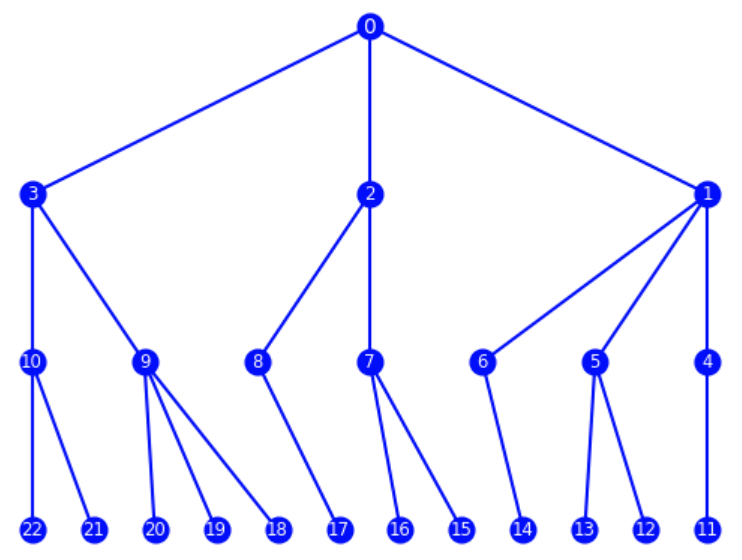
\includegraphics[scale=0.7]{images/artificial_tree_global_structure}
    \caption{Global artificial tree structure}
    \label{fig:tree_artificial_architecture}
\end{figure}

We define the true parameters of the model:
\begin{itemize}[H]
    \item The activation probabilities for each node: $\pi_k^{(\ell)}$
    \item The abundance parameters for each parent node: $\alpha_k^{(\ell)}$
\end{itemize}

Using the true parameters, we define the prior and posterior of the previous model to generate a dataset.
The following figure illustrates a sample of that dataset.
\begin{figure}[H]
    \centering
    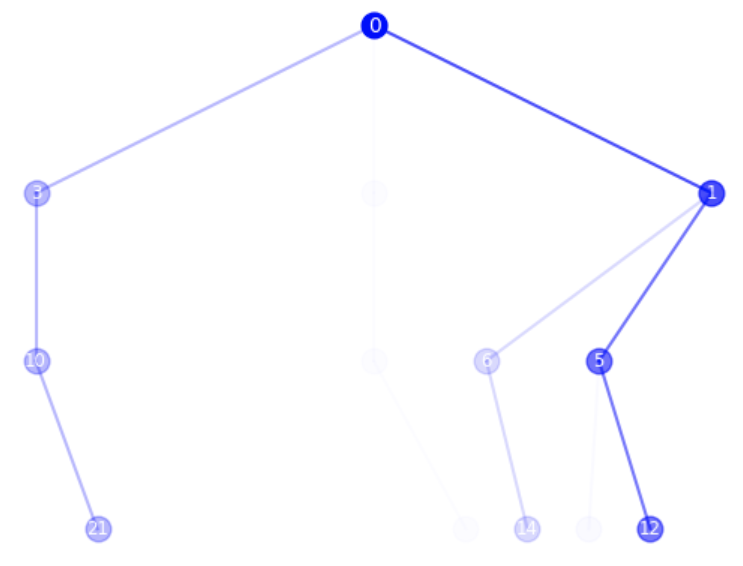
\includegraphics[scale=0.7]{images/artificial_tree_sample}
    \caption{Artificial taxa-abundance data following the global structure of figure \ref{fig:tree_artificial_architecture}.
    Opacity accounts for the value of the abundance.}
    \label{fig:tree_artificial_sample}
\end{figure}

Now that we have a dataset, we train another set of $10$ priors and posteriors onto the artifical data study the convergence of the model
and the absolute error to the parameters.
The following figure illustrates the convergence of the $10$ models for the maximum likelihood objective, relatively to the the number
of iterations done for the fixed point algorithm to compute the abundance parameters.
\begin{figure}[H]
    \centering
    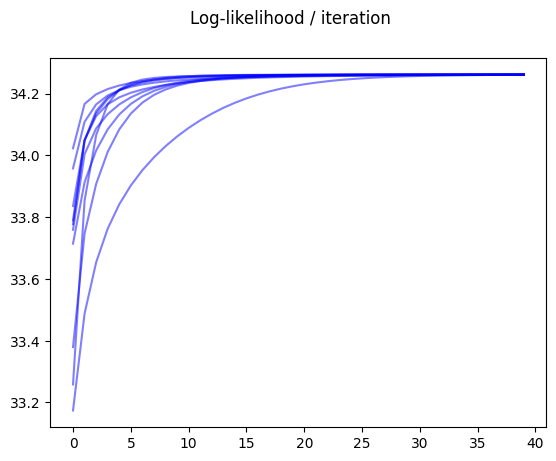
\includegraphics[scale=0.7]{images/markovian_tree_model_loglikelihood_multiple_convergences}
    \caption{Log-likelihood per iteration of the optimization algorithm for $10$ models being trained with random initializations.}
    \label{fig:markovian_tree_model_loglikelihood_convergence}
\end{figure}

Looking at figure \ref{fig:markovian_tree_model_loglikelihood_convergence}, it seems that the optimization algorithm is converging to a given $\widehat{\theta}^*$.
We would then like to compare such $\widehat{\theta}^*$ to the true set of parameters $\theta^*$.
The following figure illustrates the mean distance of the parameters to the original one: $\Vert \theta^* - \widehat{\theta}^* \Vert_2$.
\begin{figure}[H]
    \centering
    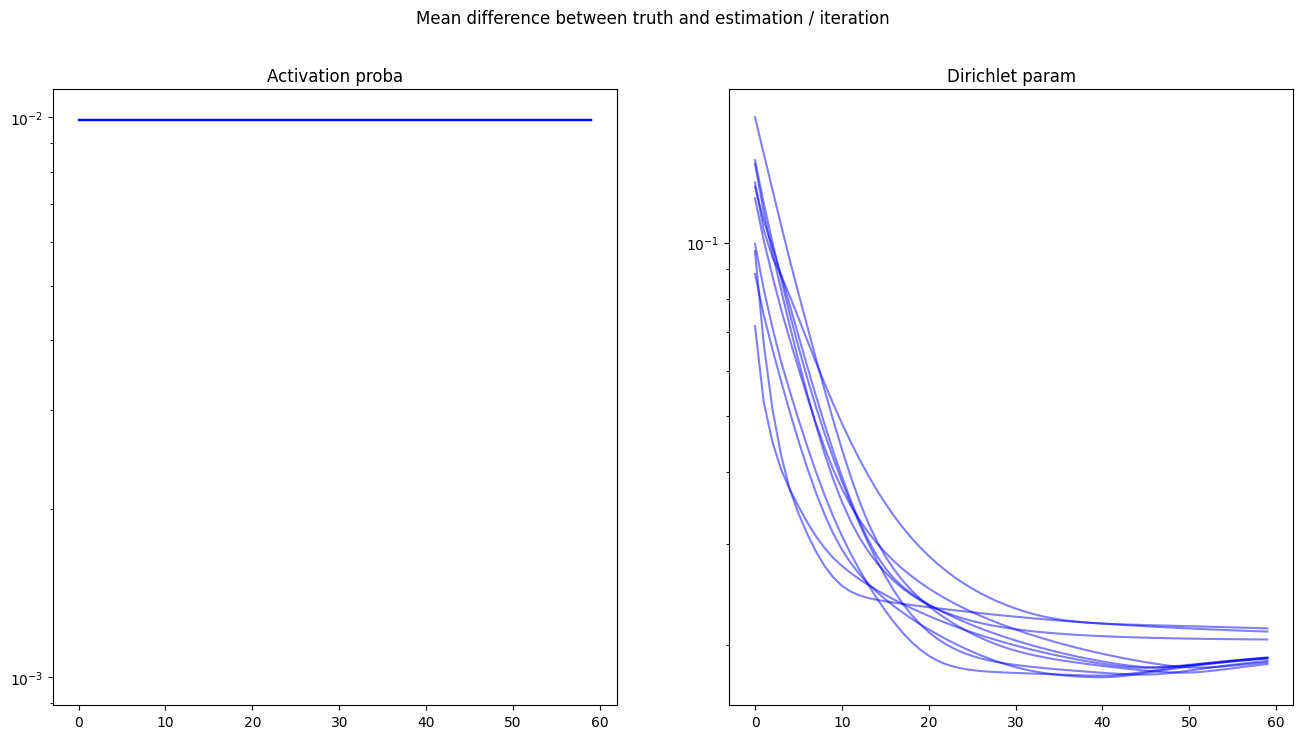
\includegraphics[scale=0.35]{images/markovian_tree_model_convergence_error_estimators_iteration}
    \caption{Average log optimization error to the real parameters for $10$ models initialized with random parameters, per iteration.}
    \label{fig:markovian_tree_model_error_convergence}
\end{figure}

Since the optimal value of $\pi_k^{(\ell)}$ is explicit, the error does not change over the iterations of the fixed point algorithm.
On the other hand, the dirichlet parameters $\alpha_k^{(\ell)}$ are optimized coordinate per coordinate in the fixed point algorithm,
leading to the convergence profile of figure \ref{fig:markovian_tree_model_error_convergence}, which shows that there is a convergence to
a given $\widehat{\theta}^*$ that is close to $\theta^*$ with mean error rate of approximately $10^{-2}$. \\

The next graph illustrates the error per coordinate of the estimated parameter and the true one for the $10$ trained models.
\begin{figure}[H]
    \centering
    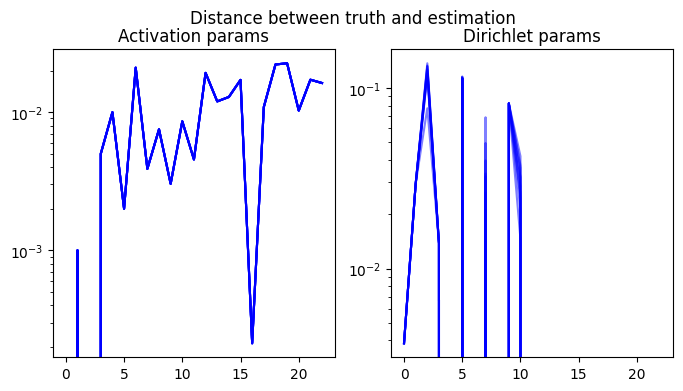
\includegraphics[scale=0.6]{images/markovian_tree_model_error_estimators}
    \caption{Coordinate-wise log optimization error to the real parameters for $10$ models initialized with random parameters, per iteration.}
    \label{fig:markovian_tree_model_error_estimations}
\end{figure}

As it seems, some coordinates are much more accurately determined than others, which highly relates to the structure of the tree (markovian)
and the general presence of each node in the dataset.
Indeed, the less likely a node is activated, the less samples we have to compute its activation probability.
Likewise, the deeper a node is in the tree, the less likely it is to be present in a tree due to the conditional probability to the parent.
That can then explain why deeper nodes are harder to grasp, and for which the parameter estimation is less good than the one of higher entities in the hierarchy of the tree. \\

Furthermore, note that we used an initialization of the $\pi_k^{(\ell)}$ to $0$, which artificially boosts the estimation quality of some node like the $16$-th one, which has a probability of activation of $0.1$
in our artificial model.
Hence, while the estimation seems to be great for that node, this is just biased by the fact that this node rarely is present and that the initialization is quite close to the truth already. \\

Finally, we look into the average optimization error as we vary the amount of samples in figure \ref{fig:markovian_tree_model_error_mean_sample}.
\begin{figure}[H]
    \centering
    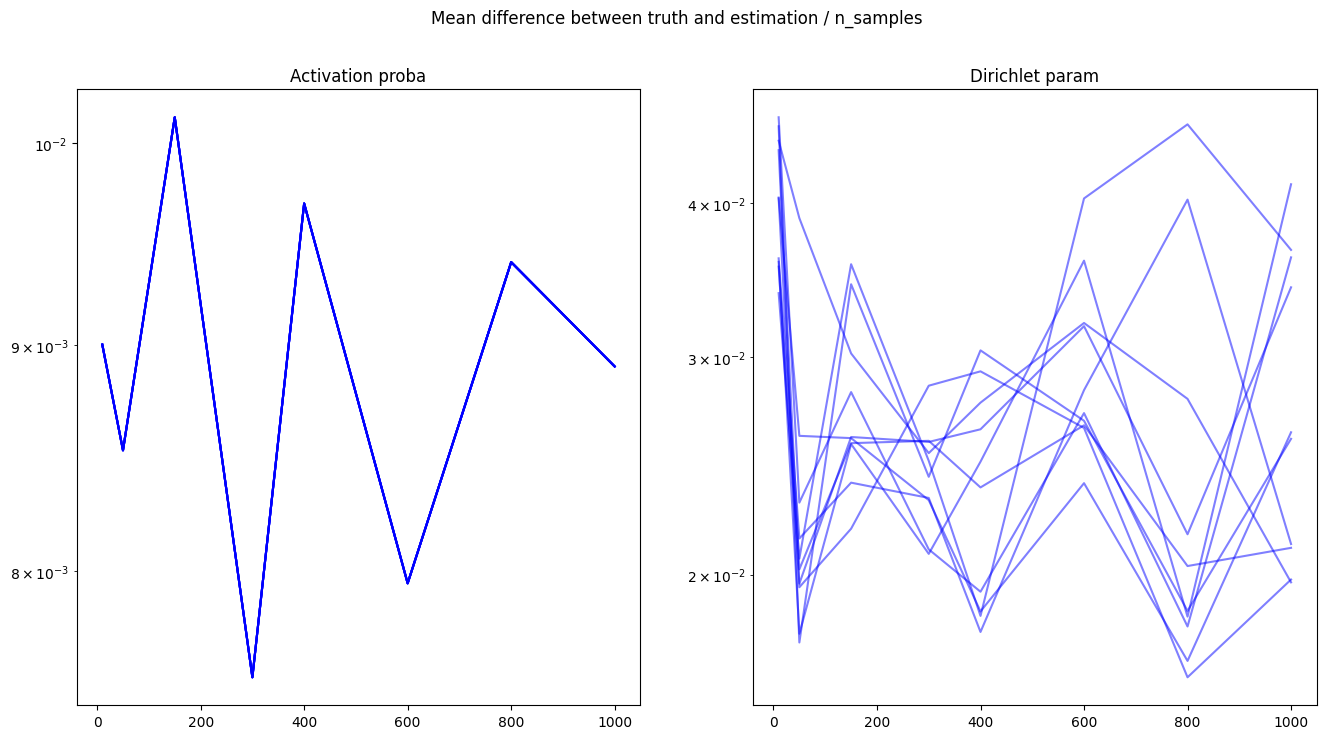
\includegraphics[scale=0.4]{images/markovian_tree_model_mean_error_samples}
    \caption{Average log optimization error to the real parameters for $10$ models initialized with random parameters, per samples in the dataset.}
    \label{fig:markovian_tree_model_error_mean_sample}
\end{figure}

As it seems, the number of samples is not impacting much the convergence towards the parameters of the models, which seems unnatural.
We would like to observe that with more samples, the variance is reducing and the estimation getting better.

\subsubsection{Conclusions}

This first model is interesting as it provides a benchmark baseline for our upcoming tree-structured models.
However, it clearly lacks of complexity:
\begin{itemize}
    \item The nodes are modeled as independent, which prevents any modelisation of correlation between entities.
          As for many ecosystems, we would expect some bacteria to have symbiotic relationship, or domination roles,
          especially when it comes to critical systems like disease detection in which some bacteria may proliferate over others.
          One idea could be to model an interaction graph (see \cite{momal_tree}) and use it as a correlation restriction between our bacteria.
    \item The abundance data generation takes the tree constraints into account, but the Dirichlet distribution is not quite expressive.
          Mixture models could enable us to provide more expressive priors and model multiple modes rather than one at the moment, to the cost of more parameters though.
    \item So far we have only considered trees without any missing entries at precision level $L$, which is not what we observe for microbiota datasets.
          Inference for missing data implementation could be interesting in the future.
\end{itemize}